%==========================================================================
% DOCUMENT
%==========================================================================

%% Document class
\documentclass[a4paper,12pt]{scrreprt}

%% Include packages
%% Used for changing margins of the document
\usepackage{geometry}
    \geometry{a4paper, top=3cm, bottom=3cm, left=3cm, right=3cm}

%% Used for special fonts
\usepackage{fontspec}
    \setmainfont{Arial}
    %% Defining sfdefault font and default font for document
    % \renewcommand{\familydefault}{\sfdefault}

%% Changes language of some packages protocols
\usepackage[portuguese]{babel}

%% More colors and color options
\usepackage[dvipsnames]{xcolor}
\usepackage{colortbl}

%% List of acronyms
\usepackage[intoc]{nomencl}
    \makenomenclature

%% More images options/settings
\usepackage{graphics}
    \graphicspath{{images}}

%% Hyperref for cross-referencing and links
\usepackage{hyperref}
%     \hypersetup{
%         colorlinks,
%         citecolor=black,
%         filecolor=black,
%         linkcolor=black,
%         urlcolor=black
%     }

%% Math environments
\usepackage{amsmath}

%% Defining backgrounds, used to make the cover
\usepackage[some]{background}

%% Used to make drawings or complex graphics
\usepackage{tikz}
    \usetikzlibrary{calc}

%% Tables with multirows and other options, like dashed/dotted lines
\usepackage{pbox, longtable, multirow, hhline, array, arydshln}

%% Include code snippets
\usepackage{listings}
    \lstset{
        captionpos=b, % Places caption below listing
        numberbychapter=true, % Optional: Number listings by chapter (4.1, 4.2, ...)
        frame=tb,
        aboveskip=3mm,
        belowskip=3mm,
        showstringspaces=false,
        columns=flexible,
        basicstyle={\small\ttfamily},
        numbers=left,
        numberstyle=\small\color{gray},
        keywordstyle=\color{blue},
        commentstyle=\color{gray},
        stringstyle=\color{Green},
        breaklines=true,
        breakatwhitespace=true,
        tabsize=4
    }
    \renewcommand{\lstlistingname}{\textit{Snippet}} % Changes "Listing" to "Snippet"

% Custom ColumnSpec for tables
\newcommand{\MyColumnSpec}{|p{0.3cm}|p{4cm}|p{3cm}|p{4.5cm}|p{3cm}|}

%% changing chapter and section title style and spacing
\usepackage{titlesec}
\titleformat{\chapter}[hang]%
  {\sffamily\Huge\bfseries}% format applied to label+text
  {\thechapter}%% label
  {0.5em}% horizontal separation between label and title body
  {}% before the title body
  []% after the title body

\titleformat{\section}[hang]%
  {\sffamily\Large\bfseries}% format applied to label+text
  {\thesection}%% label
  {0.5em}% horizontal separation between label and title body
  {}% before the title body
  []% after the title body

\titlespacing*{\chapter}{0pt}{*0}{*0}
\titlespacing*{\section}{0pt}{*0}{*0}

% Paragraph vertical spacing
% \usepackage{parskip}
% \setlength{\parskip}{5pt}


%% Include custom commands
\usepackage{commands}

\begin{document}

\pagenumbering{gobble}

%% Build cover
%% Orange cover color
\definecolor{titlepagecolor}{RGB}{47,113,187}

%==========================================================================
% COLORED BAR ON THE LEFT SIDE
%==========================================================================

\backgroundsetup{
    scale=1,
    angle=0,
    opacity=1,
    contents={
        \begin{tikzpicture}[remember picture,overlay]
            \path [fill=titlepagecolor] (-10.5,-15) rectangle ++ (5,30);
            \node[color=white] at (-7.2,-12) {\bfseries {\fontsize{120}{60} \textsf{D}}};
            \node[color=titlepagecolor] at (-4.3,-12) {\bfseries {\fontsize{120}{60} \textsf{S}}};
            \node[color=titlepagecolor] at (-2,-12) {\bfseries {\fontsize{120}{60} \textsf{S}}};
        \end{tikzpicture}
    }
}

%==========================================================================
% TITLE PAGE INFO
%==========================================================================

%% Changes values in this field to show information in the cover and back cover about your team/project

%% TITLE
\title{\LARGE{Aplicação de Gestão de Turnos}}

%% AUTHORS
\author{
    Afonso Dionísio Santos (A104276) \\
  \quad
    Afonso Gonçalves Pedreira (A104537) \\
  \quad
    Dário Silva Guimarães (A104344) \\
  \quad
    Flávia Alexandra Silva Araújo (A96587) \\
  \quad
    Miguel Torres Carvalho (A95485)
}

%% Date

\date{\today}

%% Course
\newcommand{\Course}{Licenciatura em Engenharia Informática}

%% Department
\newcommand{\Department}{Escola de Engenharia}

%% UniName
\newcommand{\UniName}{Universidade do Minho}

%% UniPic
\newcommand{\UniPic}{
\includegraphics[width=120pt]{images/eeum.png}}

%% University
\newcommand{\University}{
    \begin{flushleft}
        \UniPic
    \end{flushleft}
    \textcolor{gray}{\small\textbf{\textsf{\UniName}}}\par
    \textcolor{gray!80!white}{\small{\textsf{\Department}}}\par
    \textcolor{gray!70!white}{\small{\textsf{\Course}}}
}

%% UC
\newcommand{\UC}{
    \begin{flushleft}
        \par\textcolor{titlepagecolor}{\Large\textbf{\textsf{Desenvolvimento de Sistemas de Software}}}
    \end{flushleft}
}

%% Project Phase
\newcommand{\ProjectPhase}{
    \begin{flushleft}
        \large\textbf{Trabalho Prático - Fase 3}
    \end{flushleft}
}

%% Group Info
\newcommand{\GroupInfo}{\par Grupo 14}

%% GitHub Repo
\newcommand{\GitHubRepo}{\par\url{https://github.com/LEI-DSS/DSS2425-Grupo-14}}

%% School Year
\newcommand{\SchoolYear}{
    \par\small{\textsf{Ano Letivo de 2024/2025}}
}

%% Define new command to show title, author and date
\makeatletter
\let\Title\@title
\let\Author\@author
\let\Date\@date
\makeatother

%==========================================================================
% BEGIN COVER PAGE
%==========================================================================

% Make cover page
\newcommand{\makecover}{

%% Removes page number on footer
\thispagestyle{empty}

%% No indentation
\setlength{\parindent}{0em}

%% Put Background defined on \backgroundsetup, in this page
\BgThispage

%% Changing geometry to prevent overlay with text
%% At the end of back cover, geometry is default with \restoregeometry
\newgeometry{top=4cm,left=6cm,right=2cm,bottom=2cm}

%% builds university info defined previously
\University
\vspace{1cm}
\UC
\ProjectPhase
\GroupInfo
\GitHubRepo
\vspace{0.5cm}
\SchoolYear

\vspace*{4cm}
%% bigger space (i think its the default one) between paragraphs
\setlength{\parskip}{1em}

%% builds title info defined previously
\par\textbf{\textsf{\huge\Title}}
\vspace{1cm}
%% builds author(s) info defined previously
\par\Author

\vspace{0.5cm}

%% builds date info defined previously
\par\Date
\restoregeometry
\pagebreak

%==========================================================================
% END COVER PAGE
%==========================================================================
}

\makecover

%% Build back cover
\newcommand{\makebackcover}{

%% Removes page number on footer
\thispagestyle{empty}

\begin{center}
    \Large{\textbf{Equipa de Trabalho}}

    \vspace{1cm}

    \begin{minipage}{120pt}
        
\includegraphics[scale=0.2]{images/team/dionisio.png}
        \parbox{120pt}{\centering\normalsize{Afonso Santos \\ (A104276)}}
    \end{minipage}
    \hspace{0.5cm}
    \begin{minipage}{120pt}
        
\includegraphics[scale=0.2]{images/team/afonso.png}
        \parbox{120pt}{\centering\normalsize{Afonso Pedreira \\ (A104537)}}
    \end{minipage}
    \hspace{0.5cm}
    \begin{minipage}{120pt}
        
\includegraphics[scale=0.2]{images/team/dario.png}
        \parbox{120pt}{\centering\normalsize{Dário Guimarães \\ (A104344)}}
    \end{minipage}

    \vspace{0.5cm}

    \begin{minipage}{120pt}
        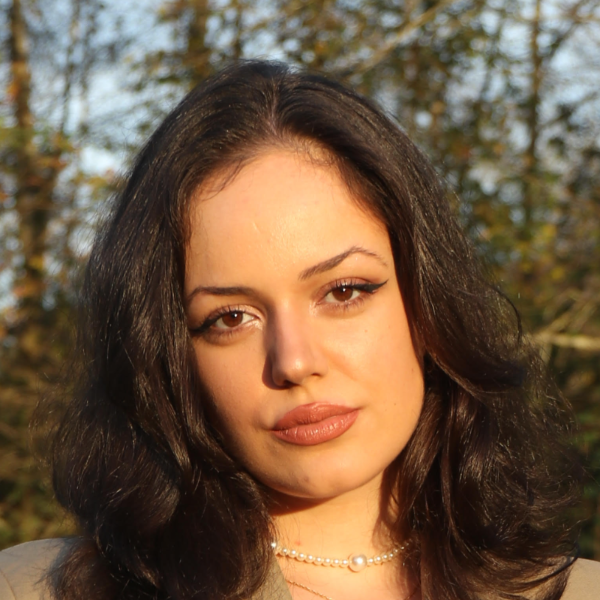
\includegraphics[scale=0.2]{images/team/flavia.png}
        \parbox{120pt}{\centering\normalsize{Flávia Araújo \\ (A96587)}}
    \end{minipage}
    \hspace{0.5cm}
    \begin{minipage}{120pt}
        
\includegraphics[scale=0.2]{images/team/miguel.png}
        \parbox{120pt}{\centering\normalsize{Miguel Carvalho \\ (A95485)}}
    \end{minipage}
\end{center}

\pagebreak

}

\makebackcover

%% Default geometry
\newgeometry{top=2cm,left=3cm,right=3cm,bottom=3.5cm}

%% Save default geometry
\savegeometry{default}

%% Load default geometry with:
% \loadgeometry{default}

%==========================================================================
% BEGIN ABSTRACT PAGE
%==========================================================================

%% Abstract name: \Large font size, flushed left and paragraph skip before abstract content
% \renewenvironment{abstract}
%  {\par\noindent\textbf{\Large\abstractname}\par\bigskip}
%  {}
%
% \begin{flushleft}
% \begin{abstract}
%     Exemplo
%
%     \textbf{Área de Aplicação}: Exemplo
%
%     \textbf{Palavras-Chave}: Exemplo
%
% \end{abstract}
% \end{flushleft}
%
% \pagebreak

%==========================================================================
% END ABSTRACT PAGE
%==========================================================================

%==========================================================================
% BEGIN INDEXES PAGES
%==========================================================================

%% Changes table of content name
\renewcommand{\contentsname}{Índice}
\renewcommand{\listfigurename}{Índice de Figuras}
\renewcommand{\listtablename}{Índice de Tabelas}

\tableofcontents

\pagebreak

\listoffigures

\pagebreak

% \listoftables
%
% \pagebreak

%==========================================================================
% END INDEXES PAGES
%==========================================================================

%==========================================================================
% BEGIN ATUALIZAÇÔES REFERENTES À PRIMEIRA FASE
%==========================================================================

\chapter{Atualizações Referentes à Primeira Fase}
\vspace{1cm}

Relativamente à primeira fase do projeto, foram realizadas as seguintes atualizações:

\begin{itemize}
    \item \textbf{Modelo de Análise}: Adição dos relacionamentos entre Aluno e Horário, e
        entre Diretor de Curso e Horário.
    \item \textbf{Especificações de \textit{Use Cases}}: Renomeação do \textit{use case}
        “Instalar aplicação” para “Primeira configuração”, com a sua generalização para
        arquiteturas sem persistência de dados. Alteração dos termos “Aluno” e “Diretor de Curso”
        para “Utilizador” e “Ator”, de forma a generalizar os casos de uso.
    \item \textbf{Diagramas de \textit{Use Cases}}: Renomeação do \textit{use case}
        “Instalar aplicação” para “Primeira configuração”.
\end{itemize}

%==========================================================================
% END ATUALIZAÇÔES REFERENTES À PRIMEIRA FASE
%==========================================================================

%==========================================================================
% BEGIN MODELO DE ANÁLISE
%==========================================================================

%% Starting page numbering here
\pagenumbering{arabic}

\chapter{Modelo de Análise}
\vspace{2cm}

\begin{minipage}{\textwidth}
    \centering
    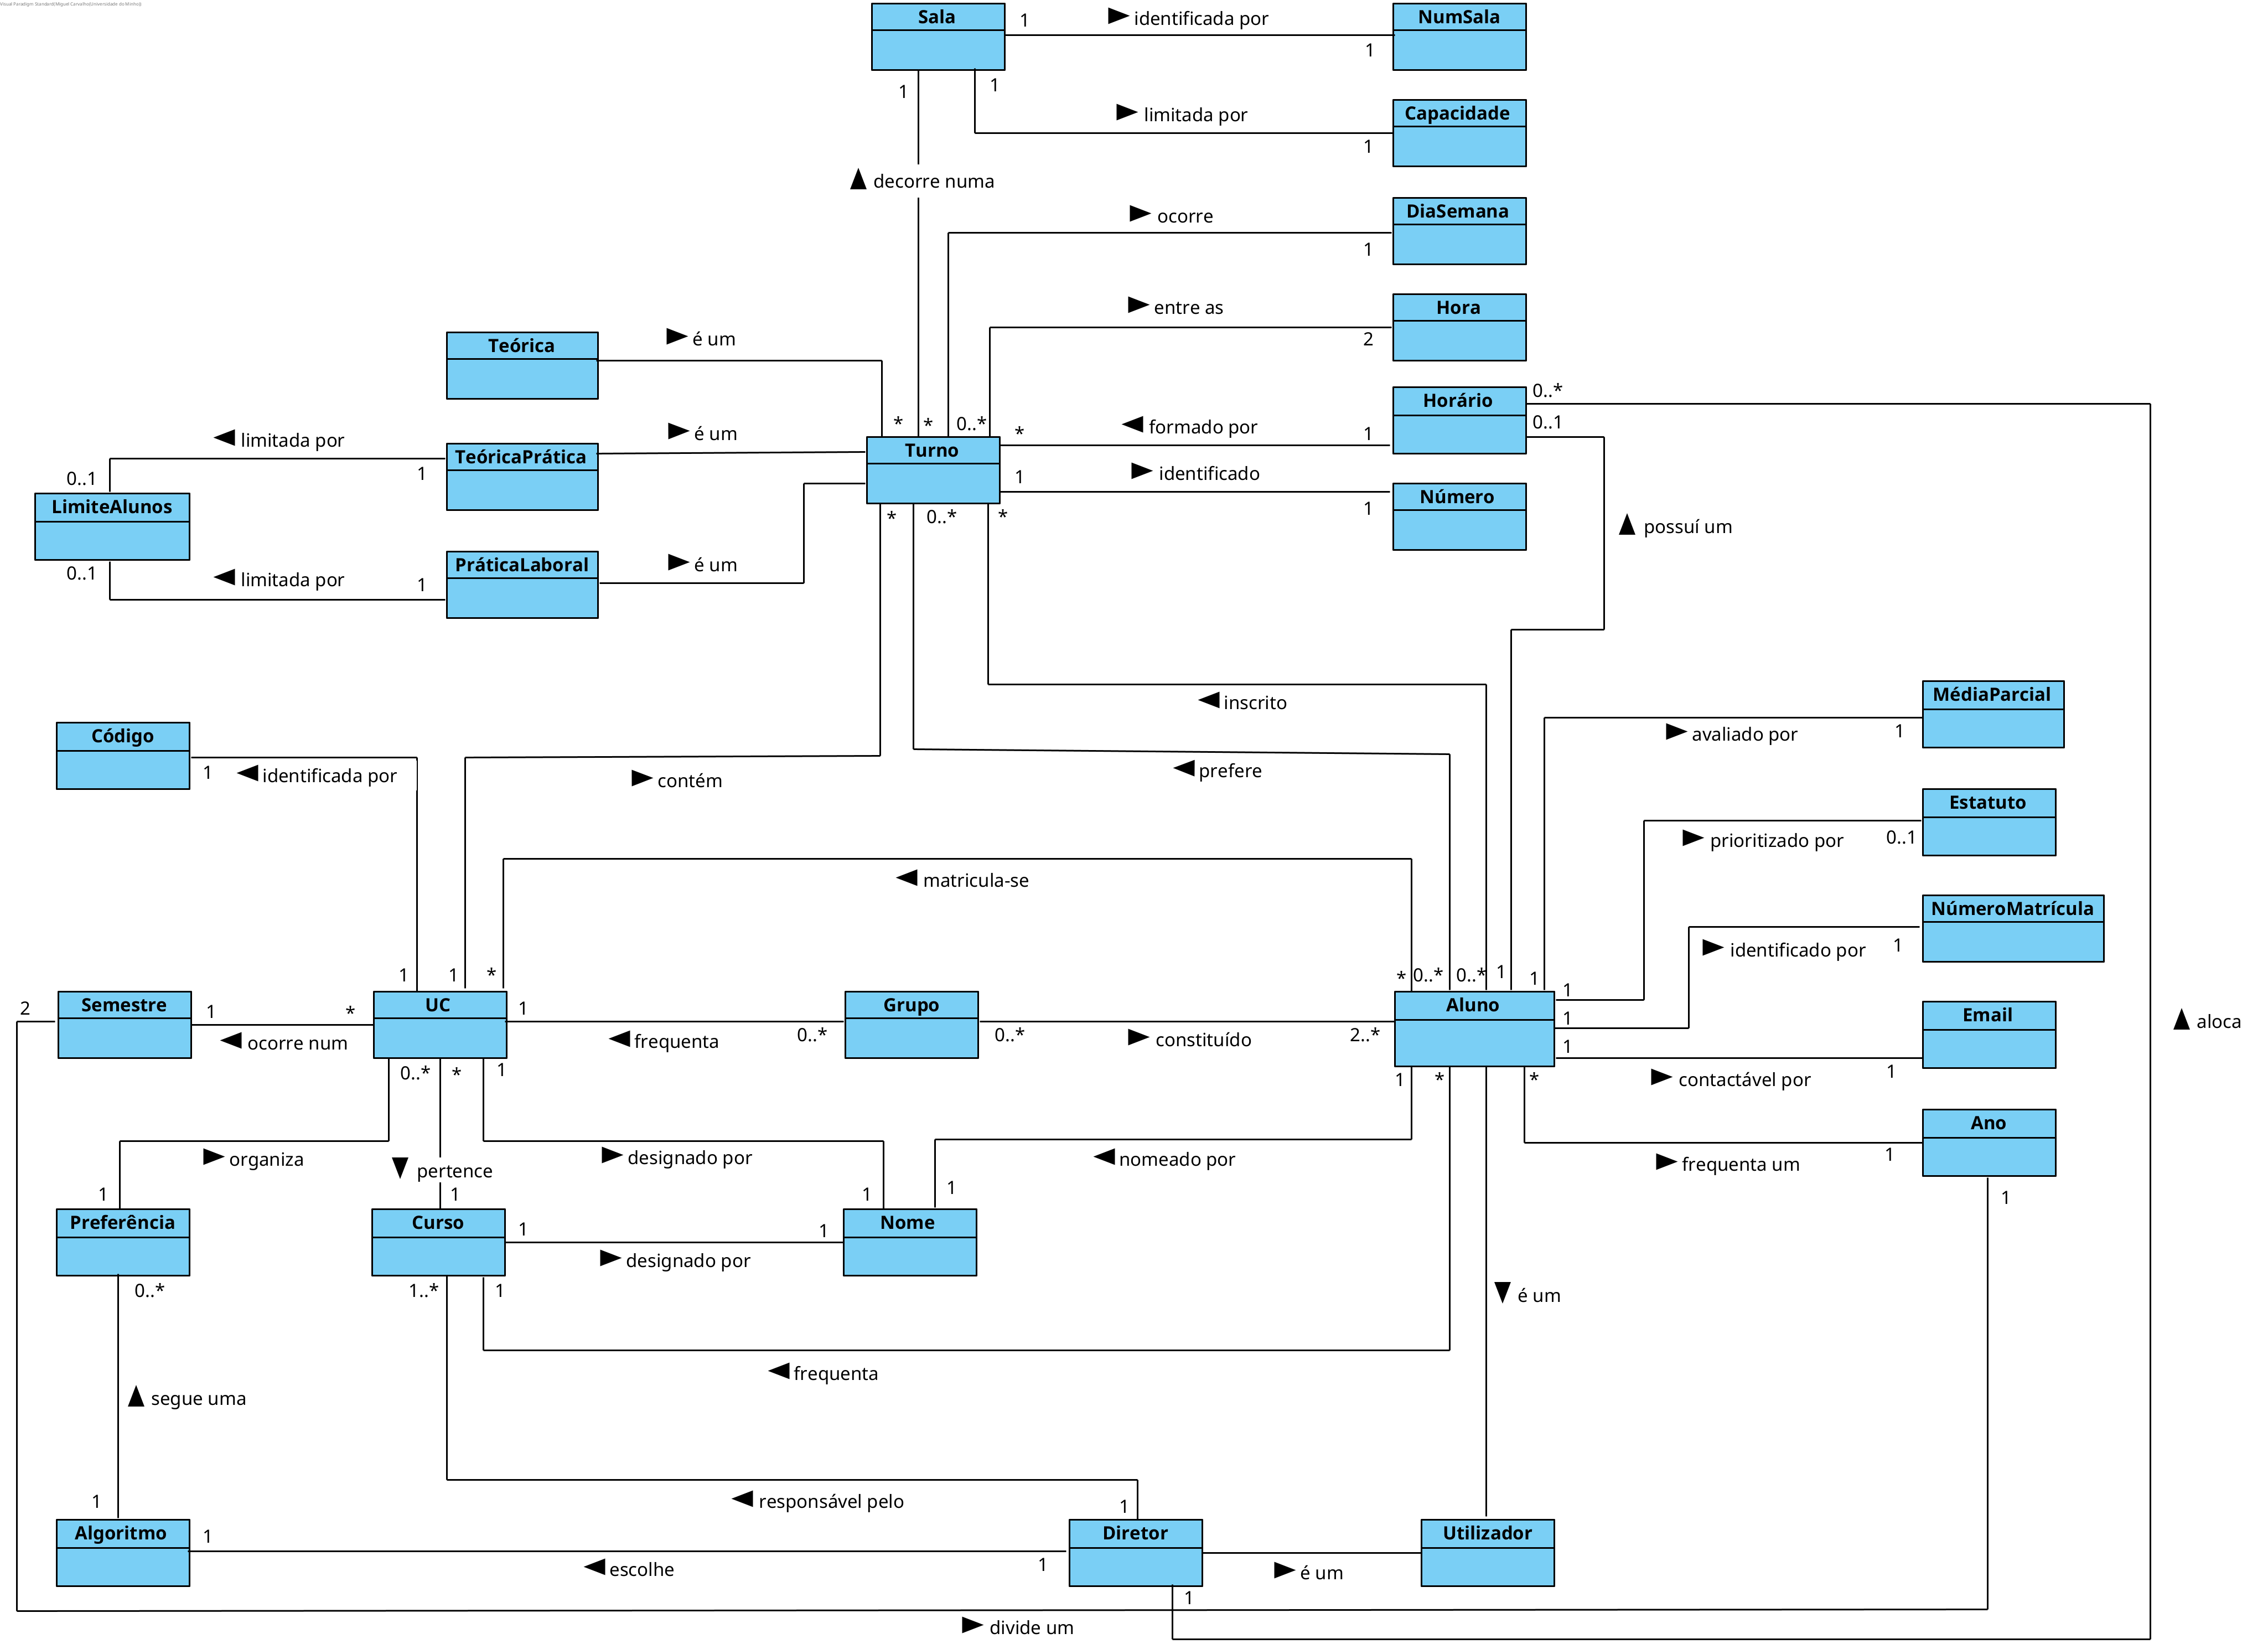
\includegraphics[width=1\textwidth]{images/modelo-analise.png}
    \captionof{figure}{Modelo de Análise}
    \label{fig:modelo_analise}
\end{minipage}

%==========================================================================
% END MODELO DE ANÁLISE
%==========================================================================

%==========================================================================
% BEGIN DIAGRAMAS DE CASOS DE USO
%==========================================================================

\chapter{Diagramas de Casos de Uso}
\vspace{1cm}

\begin{minipage}{\textwidth}
    \centering
    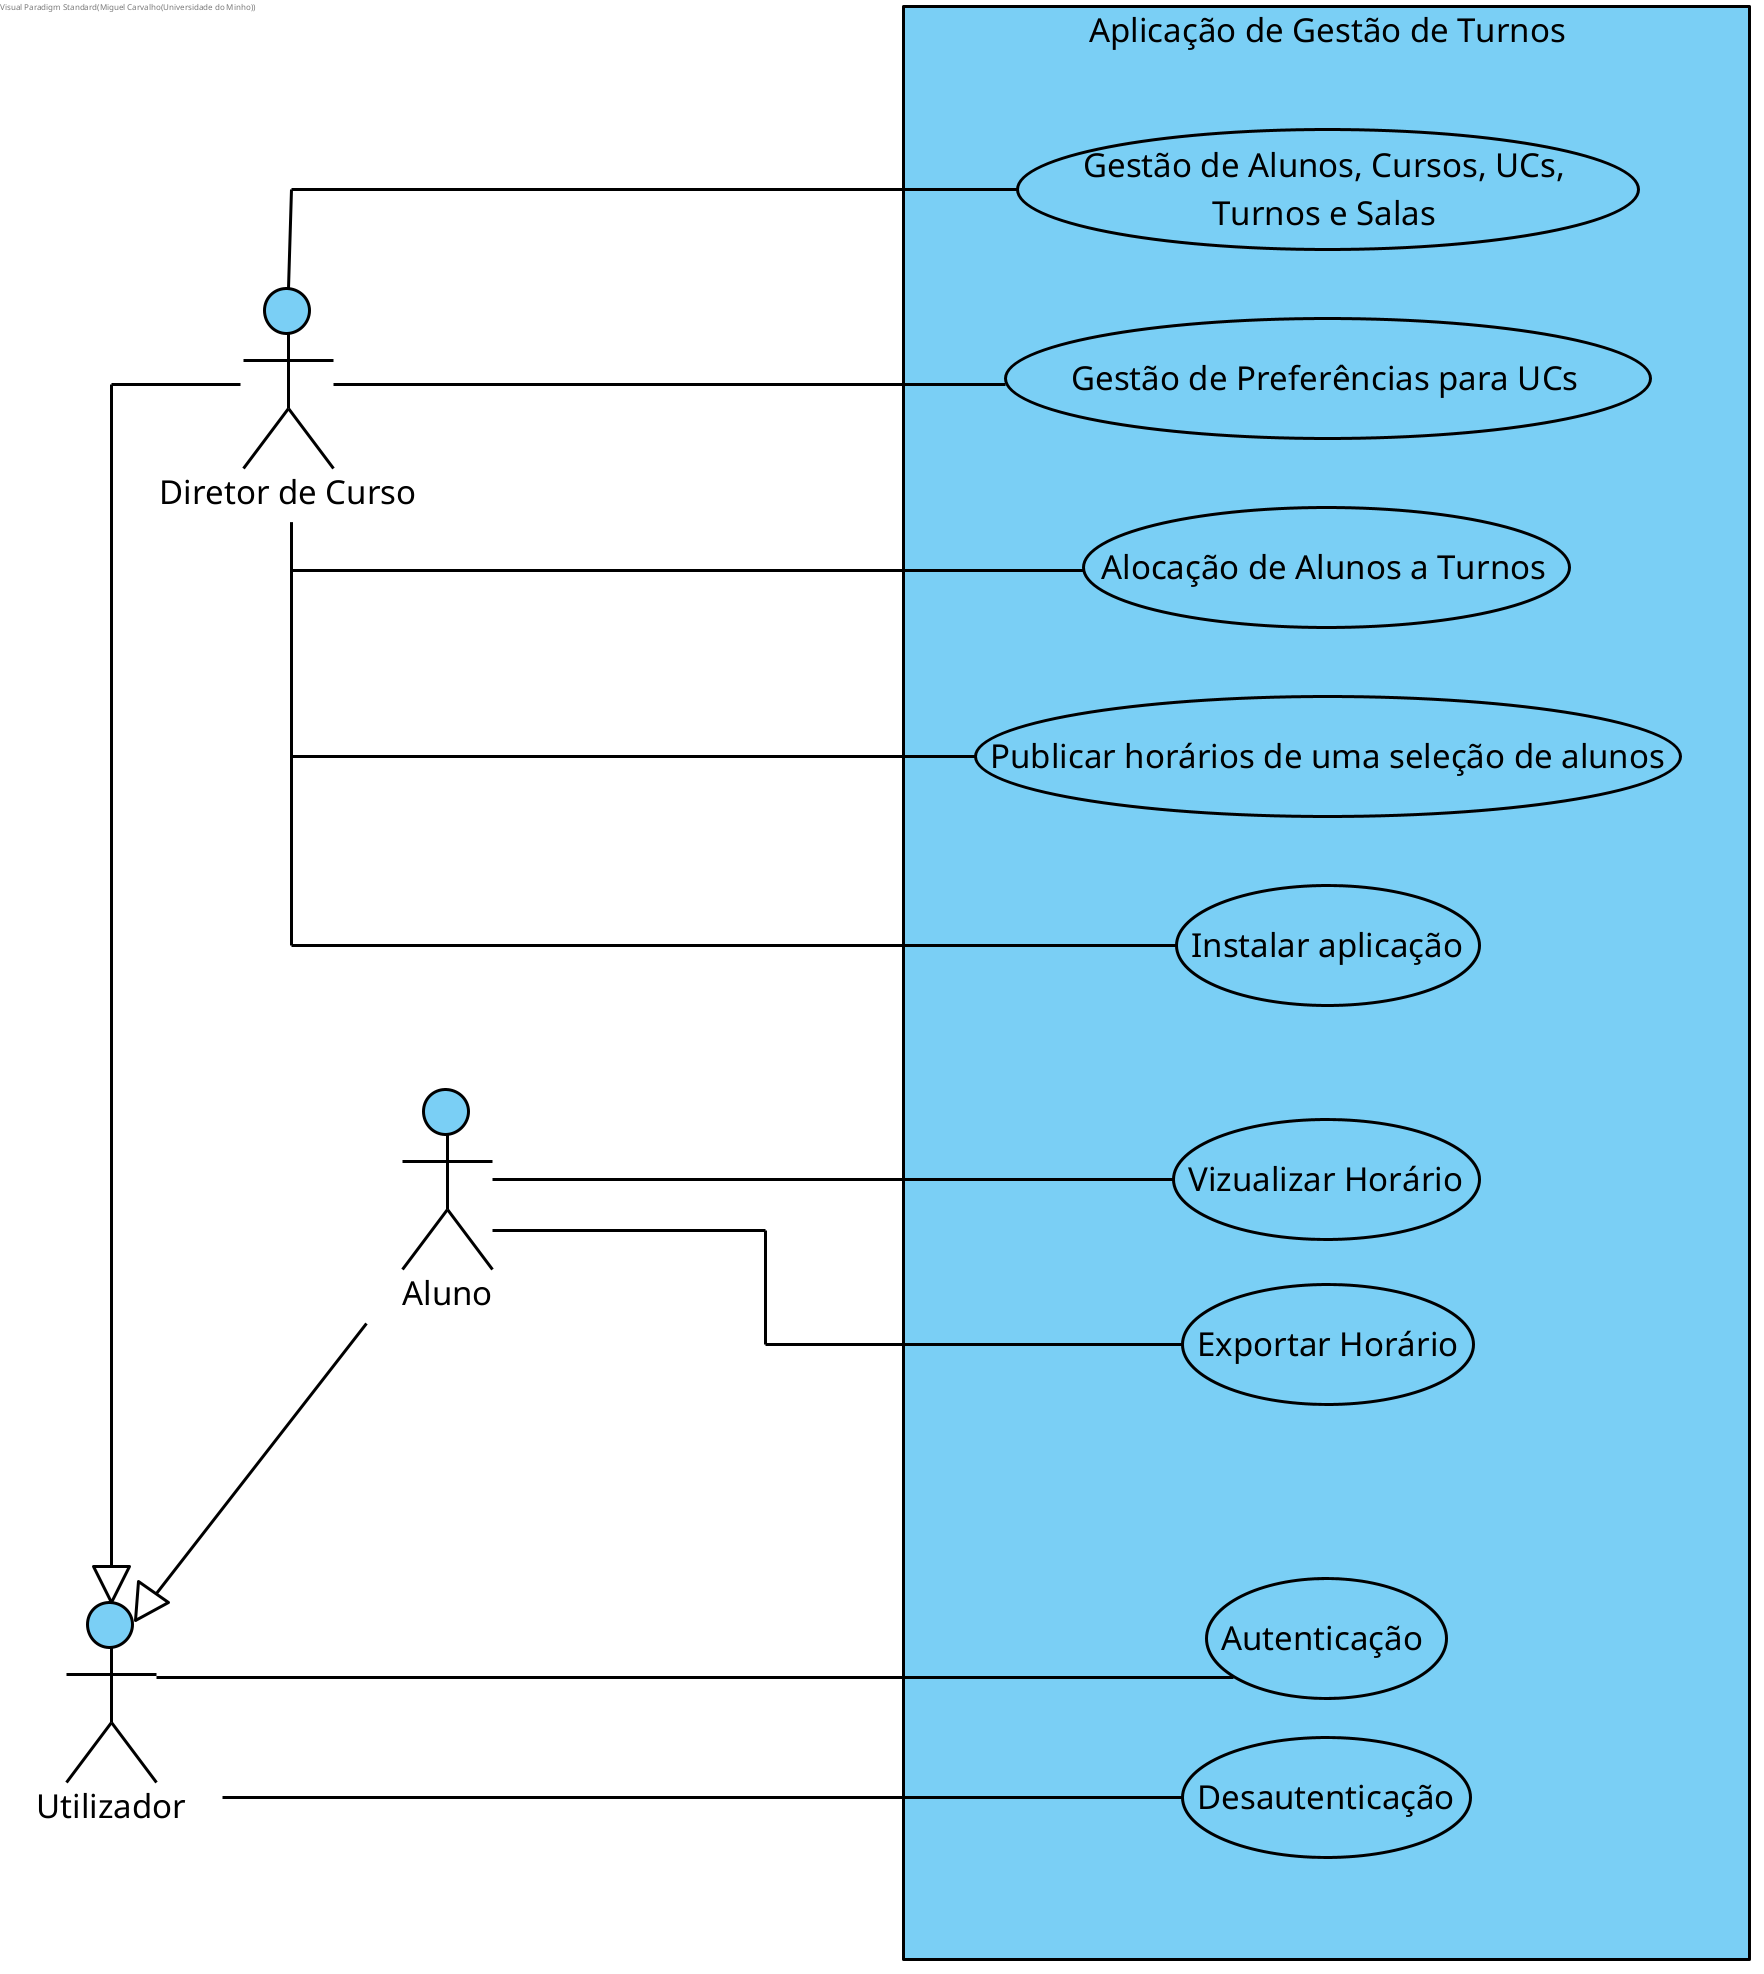
\includegraphics[width=1\textwidth]{images/use-cases/diagrams/1-geral.png}
    \captionof{figure}{Diagrama de Casos de Uso - Geral}
    \label{fig:2-1-diagrama_de_casos_de_uso_geral}
\end{minipage}

\begin{minipage}{\textwidth}
    \centering
    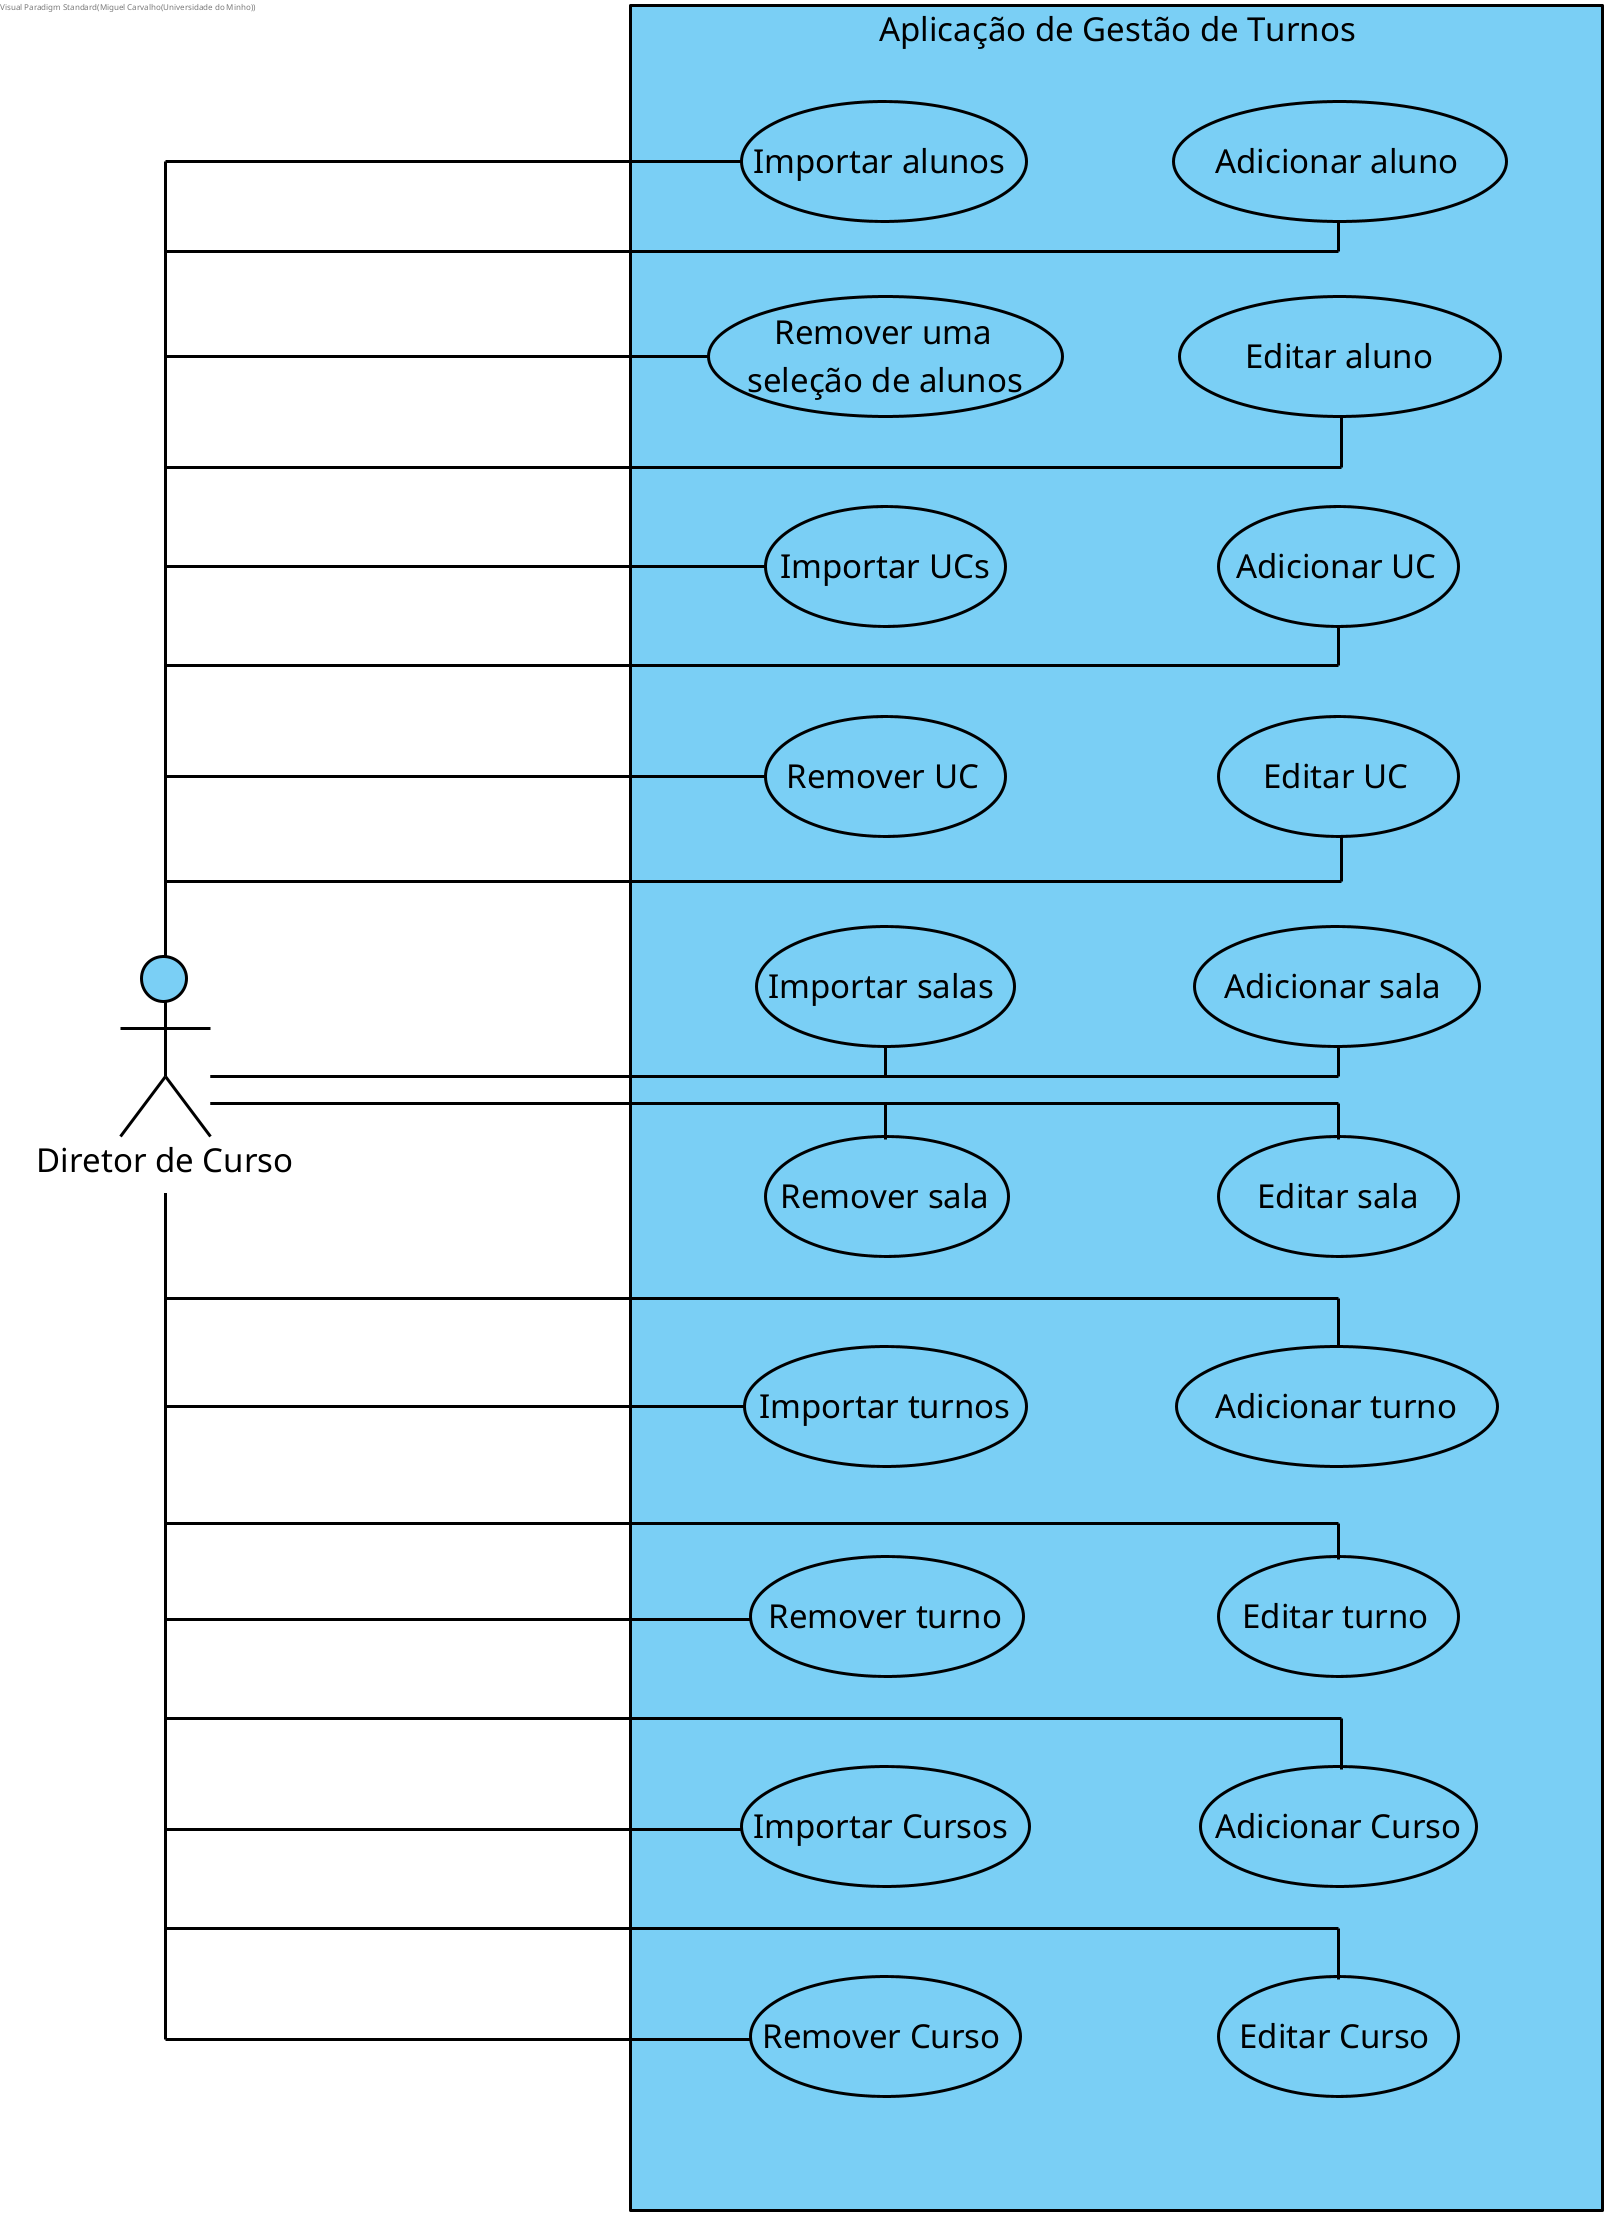
\includegraphics[width=1\textwidth]{images/use-cases/diagrams/2-gestao-alunos-cursos-ucs-turnos-salas.png}
    \captionof{figure}{Diagrama de Casos de Uso - Gestão de Alunos, Cursos, UCs, Turnos e Salas}
    \label{fig:2-2-diagrama_de_casos_de_uso_gestao_de_alunos_cursos_ucs_turnos_e_salas}
\end{minipage}

\begin{minipage}{\textwidth}
    \centering
    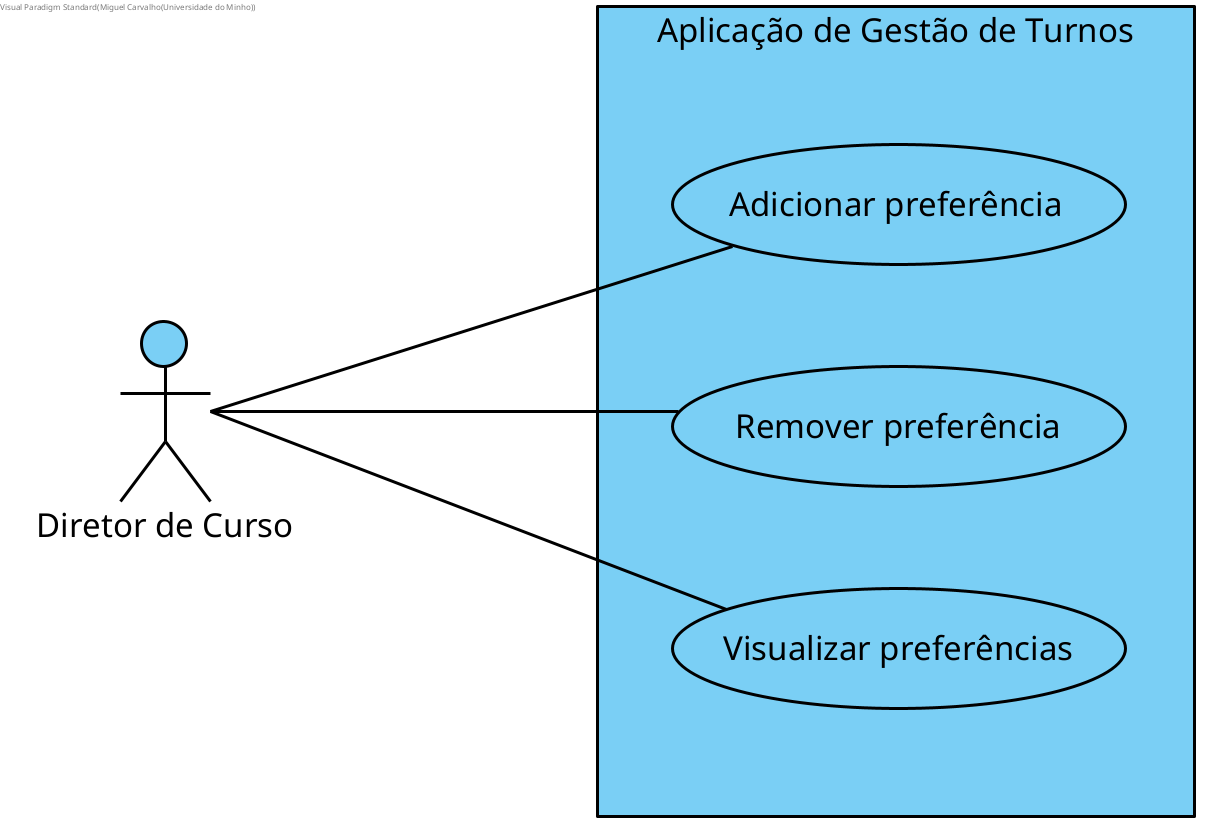
\includegraphics[width=1\textwidth]{images/use-cases/diagrams/3-gestao-preferencias.png}
    \captionof{figure}{Diagrama de Casos de Uso - Gestão de Preferências para UCs}
    \label{fig:2-3-diagrama_de_casos_de_uso_gestao_de_preferencias}
\end{minipage}

\vspace{1cm}

\begin{minipage}{\textwidth}
    \centering
    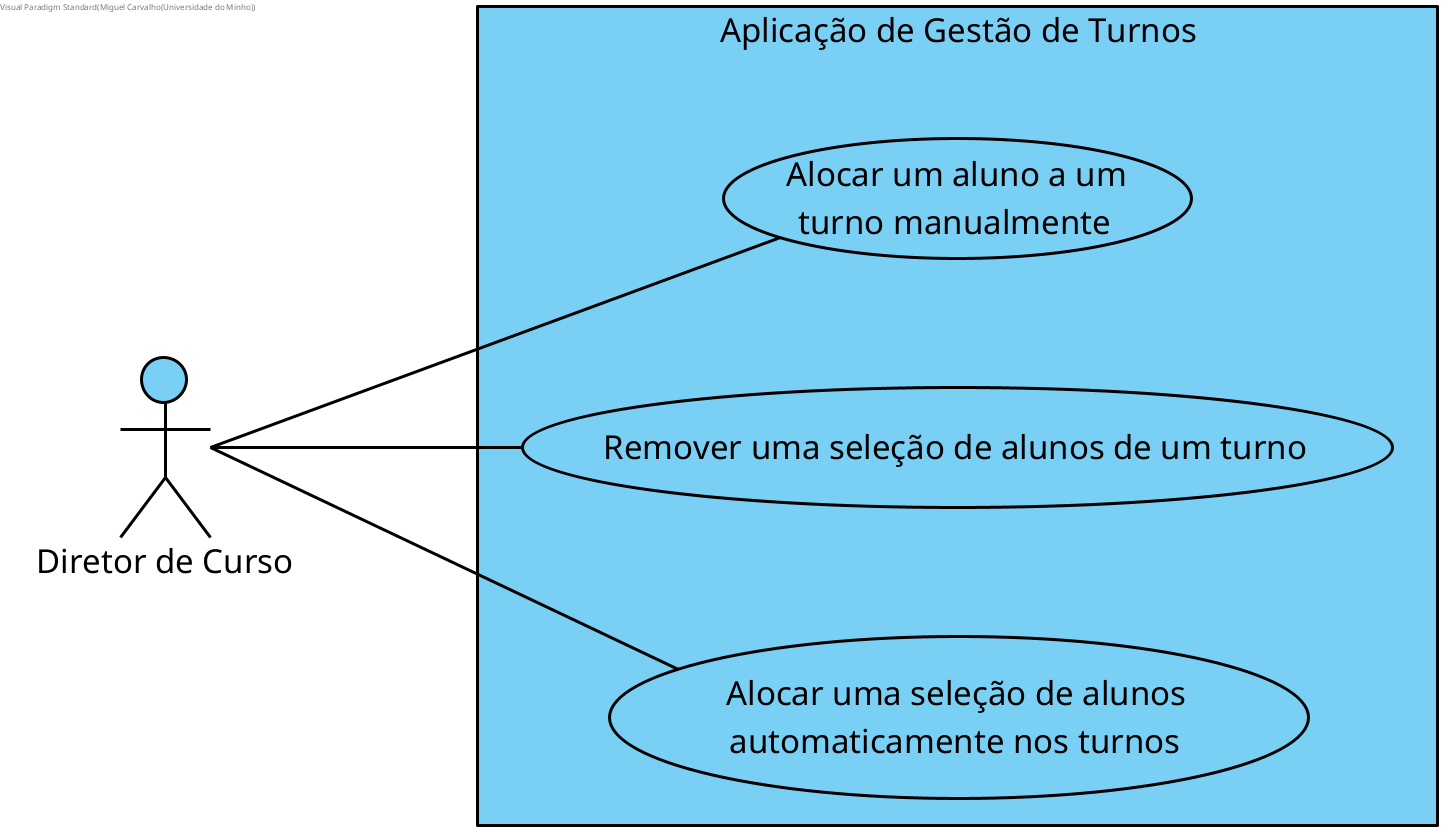
\includegraphics[width=1\textwidth]{images/use-cases/diagrams/4-alocacao-alunos.png}
    \captionof{figure}{Diagrama de Casos de Uso - Alocação de Alunos a Turnos}
    \label{fig:2-4-diagrama_de_casos_de_uso_alocacao_de_alunos}
\end{minipage}

%==========================================================================
% END DIAGRAMAS DE CASOS DE USO
%==========================================================================

%==========================================================================
% BEGIN ESPECIFICAÇÕES DE CASOS DE USO
%==========================================================================

\chapter{Especificações de Casos de Uso}
\vspace{1cm}

\textcolor{red}{As especificações de casos de uso encontram-se em anexo TODO, com as respetivas,
identificações das responsabilidades da lógica de negócio, definições da API e
subsistemas envolvidos.}

%==========================================================================
% END ESPECIFICAÇÕES DE CASOS DE USO
%==========================================================================

%==========================================================================
% BEGIN DIAGRAMA DE COMPONENTES
%==========================================================================

\chapter{Diagrama de Componentes}
\vspace{1cm}

\textcolor{red}{TODO}

%==========================================================================
% END DIAGRAMA DE COMPONENTES
%==========================================================================

%==========================================================================
% BEGIN DIAGRAMA DE CLASSES
%==========================================================================

\chapter{Diagrama de Classes}
\vspace{1cm}

\textcolor{red}{TODO}

%==========================================================================
% END DIAGRAMA DE CLASSES
%==========================================================================

%==========================================================================
% BEGIN DIAGRAMA DE PACOTES
%==========================================================================

\chapter{Diagrama de Pacotes}
\vspace{1cm}

\textcolor{red}{TODO}

%==========================================================================
% END DIAGRAMA DE PACOTES
%==========================================================================

%==========================================================================
% BEGIN DIAGRAMAS DE SEQUÊNCIA
%==========================================================================

\chapter{Diagramas de Sequência}
\vspace{1cm}

\textcolor{red}{TODO}

%==========================================================================
% END DIAGRAMAS DE SEQUÊNCIA
%==========================================================================

%==========================================================================
% BEGIN DIAGRAMA DE INSTALAÇÃO
%==========================================================================

\chapter{Diagrama de Instalação}
\vspace{1cm}

\textcolor{red}{TODO}

%==========================================================================
% END DIAGRAMA DE INSTALAÇÃO
%==========================================================================

%==========================================================================
% BEGIN CONSIDERAÇÕES PERTINENTES
%==========================================================================

\chapter{Considerações Pertinentes}
\vspace{1cm}

Ao longo dos casos de uso apresentados, foi utilizado o termo “seleção de alunos”.
Este termo refere-se a um conjunto de alunos que foram selecionados com base em critérios específicos,
como por exemplo, alunos de um determinado ano, unidade curricular, com estatuto, entre outros.

Esta generalização permite que os casos de uso sejam mais flexíveis
e possam ser aplicados a diferentes situações. Como por exemplo, a alocação de somente
um aluno, selecionado atráves do seu número, a um turno.

A seleção de alunos também permite ao Diretor de Curso a definição da ordem
a qual os alunos devem ser alocados a turnos.

\vspace{1cm}

Caso a monotorização de atividades, através de um sistema de \textit{logs}, fosse um requisito funcional,
desejado pela equipa docente, seria possível adicionar um caso de uso que permitisse a visualização
de \textit{logs} de atividade, como por exemplo, a data e hora de criação de um turno,
ou a data e hora de alocação de um aluno a um turno. Para tal, seria necessário
incorporar esta ação do sistema nos casos de uso, nos quais se justificaria registar tal ação.

%==========================================================================
% END CONSIDERAÇÕES PERTINENTES
%==========================================================================

%==========================================================================
% BEGIN BIBLIOGRAFIA
%==========================================================================

%% Changes biblibography name
%% Portuguese babel default : “Bibliografia”
%% Personally I prefer “Referências”
% \renewcommand\bibname{Referências}

%% https://www.overleaf.com/learn/latex/bibliography_management_with_bibtex
% \begin{thebibliography}{9}
% \bibitem{DatabaseSystems}
% Connolly, T., \& Begg, C. (2015). Database Systems: A Practical Approach to Design, Implementation, and Management (6th ed.). Pearson Education. London, UK.
%
% \bibitem{Aprendizagem em Banco de Dados}
% Cândido, C. H. (2005). Aprendizagem em Banco de Dados: Implementação de Ferramenta de Modelagem E.R. Monografia de Especialização. Universidade Federal de Santa Catarina, Brasil.
%
% \bibitem{MySQLManual}
% MySQL 8.0 Reference Manual (2024). \href{https://dev.mysql.com/doc/refman/8.0/en/storage-requirements.html}{\underline{MySQL 8.0 Reference Manual: Data Type Storage} \underline{Requirements}}. MySQL, Oracle.
% \end{thebibliography}

%% Add bibliografia to index
% \addcontentsline{toc}{chapter}{Bibliografia}

%==========================================================================
% END BIBLIOGRAFIA
%==========================================================================

%==========================================================================
% BEGIN LISTA DE SIGLAS E ACRÓNIMOS
%==========================================================================

%% Portuguese babel does not translate this environment
\renewcommand{\nomname}{Lista de Siglas e Acrónimos}

%% acronyms
\nomenclature[01]{\textbf{BD}}{Base de Dados}
\nomenclature[02]{\textbf{SBD}}{Sistema de Base de Dados}

%% Show acronyms
% \printnomenclature

%==========================================================================
% END LISTA DE SIGLAS E ACRÓNIMOS
%==========================================================================

%==========================================================================
% BEGIN ANEXOS
%==========================================================================
%
%% Why \addchap, instead of \chapter?
%% \addchap has no numbering but appears in table of contents.
% \addchap{Anexos}
%
%     \addsec{
%         \href{https://docs.google.com/spreadsheets/d/1o4Pl00OfLMH4ukDdvNz3TweH2OxFpA7t8Vd_v-Idx-c/edit?usp=sharing}{\small [I] Diagrama de Gantt}
%         \label{anexo:1}
%     }
%
%     \addsec{
%         \href{https://docs.google.com/spreadsheets/d/1ZYYOut1zsdGr3DZ1JqruOHxCBgM_EFV9JDmxPFWZpiY/edit?usp=sharing}{\small [II] Documentos de Requisitos}
%         \label{anexo:2}
%     }

%==========================================================================
% END ANEXOS
%==========================================================================
\end{document}
